\documentclass[12pt,a4paper]{report}
\usepackage[brazil]{babel}
\usepackage[]{algorithm}
\usepackage[]{algorithmic}

\usepackage[style=numeric,backend=biber]{biblatex}
\usepackage[utf8]{inputenc}
\usepackage{kpfonts}
\usepackage[T1]{fontenc}
\usepackage{wrapfig}
\usepackage{graphicx}
\usepackage{enumerate}
\usepackage{subcaption}
\usepackage{float}
\usepackage{caption}
\usepackage{listings}
\usepackage{lipsum}
\usepackage{amsthm}
\usepackage{amssymb}
\usepackage{bm}
\usepackage{color}
\usepackage{afterpage}
\usepackage[inline]{enumitem}
\usepackage{pdflscape}
\usepackage{listingsutf8}
\usepackage{siunitx}
\usepackage{bashful}

\usepackage{hyperref}
\hypersetup{
    colorlinks=true,
    linkcolor=blue,
    filecolor=magenta,      
    urlcolor=cyan,
}

\usepackage[margin=1in]{geometry}

\lstset{frame=tb,
  aboveskip=2mm,
  belowskip=2mm,
  showstringspaces=false,
  columns=flexible,
  basicstyle=\footnotesize,,
  numbers=left,
  numbersep=5pt,
  stepnumber=1,
  breaklines=true,
  keepspaces=true,
  breakatwhitespace=true,
  showtabs=false,  
  tabsize=2
}


% Definindo estilo para os códigos
\definecolor{mGreen}{rgb}{0,0.6,0}
\definecolor{mGray}{rgb}{0.5,0.5,0.5}
\definecolor{mPurple}{rgb}{0.58,0,0.82}
\definecolor{dkgreen}{rgb}{0,0.6,0}
\definecolor{backgroundColour}{rgb}{0.97,0.97,0.97}

\lstset{basicstyle=\ttfamily,
    backgroundcolor=\color{backgroundColour},   
    commentstyle=\color{mGreen},
    keywordstyle=\color{magenta},
    numberstyle=\tiny\color{mGray},
    commentstyle=\color{dkgreen},
    stringstyle=\color{mPurple},
    basicstyle=\footnotesize,
    breakatwhitespace=false\textbf{,}         
    breaklines=true,                 
    captionpos=b,                    
    keepspaces=true,                 
    numbers=left,                    
    numbersep=5pt,                  
    showspaces=false,                
    showstringspaces=false,
    showtabs=false,                  
    tabsize=2,
    language=bash
}

\lstdefinestyle{BStyle}{
    backgroundcolor=\color{backgroundColour},  
    showstringspaces=false,
    numbers=none,
    language=bash
}

\pagenumbering{arabic}
\renewcommand{\thesection}{\arabic{section}}

\bibliography{ref}
\renewcommand{\contentsname}{Sumário}{\thispagestyle{empty}}
\renewcommand{\baselinestretch}{1.5} 

\begin{document}

\begin{titlepage}
        \begin{center}
                \vspace*{1cm}
                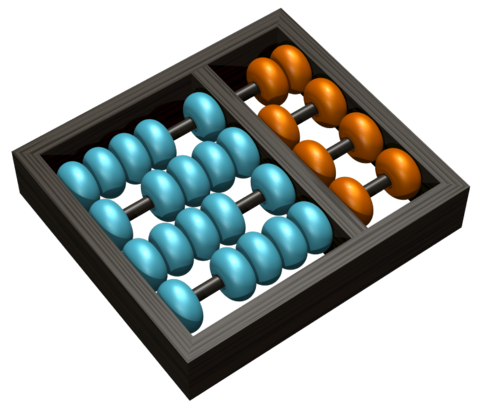
\includegraphics[width=0.25\textwidth]{Logo}\\
                \vspace{1.5cm}
                \Huge
                \textbf{Exercício 3}\\
                \vspace{1.5cm}
                \Large
                \textbf{Aluno}: João Vitor Gonçalves\\
                \textbf{RA}: 176353\\
                \vspace{1.2cm}
                \Large
                Instituto de Computação\\
                Universidade Estadual de Campinas\\
                \vspace{1.5cm}
                Campinas, 17 de Novembro de 2020.
        \end{center}
\end{titlepage}
\tableofcontents
\clearpage

\newcommand{\shellcmd}[1]{\texttt{\footnotesize\# #1}}%estilizando citação de comandos do shell

\section{Com o conhecimento adquirido em aula explique qual a relação entre backlog e
número de conexões.}

O backlog se refere ao tamanho somado de duas filas de conexão: A fila de conexões que foram estabelecidas e ainda estão ativas, e a fila de conexões pendentes.

Então o servidor pode ter tantas conexões concorrentes quanto o tamanho do backlog permitir.

Porém o valor passado no parâmetro \emph{backlog} na chamada \emph{listen} não corresponde exatamente à esse mesmo tamanho 
das filas. Cada versão de sistema operacional pode interpretar esse valor passado de e definir o tamanho do backlog real de formas diferentes.


% Relação entre backlog e número de conexões:
% Backlog: soma duas filas: filas das conexões que foram estabelecidas corretamente e estão ativas, e a fila das conexões pendentes.

% Valor passado no parâmetro backlog não corresponde necessáriamente ao tamanho do mesmo (depende de OS par OS)

% Servidor ignore SYNs quando fila está cheia

\section{Pesquise como está implementado o backlog de um socket TCP no kernel linux (para
versão 2.2 ou mais recentes), e em seguida indique o valor padrão do backlog.
Comprove sua resposta através de figuras no seu relatório.}

À partir da versão 2.2, o comportamento do backlog foi alterado. Antes ele determinava o tamanho máximo da fila de conexões aguardando um \emph{SYN}, ou seja, o número de conexões incompletas pendentes.

Porém após a versão 2.2, o \emph{backlog} determina o número da fila de conexões no estado \emph{ESTABLISHED}, ou seja, conexões que já passaram pelo \emph{handshake} (\emph{SYN} e \emph{SYN ACK}), e estão aguardando por um \emph{accept}.

\begin{figure}[H]
  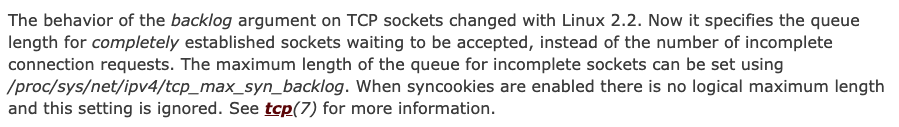
\includegraphics[width=\linewidth]{backlog-22.png}
  \caption{Man do comando listen.}
\end{figure}

Então existem dois tamanhos de fila no linux, uma definida pelo sistema para conexões aguardando \emph{SYN} e uma fila para o \emph{accept}.

No caso da fila de \emph{SYN} estar cheia, o kernel irá simplesmente ignorar novas conexões, e no caso da fila de \emph{accept} estar cheia, pacotes enviados pela conexão que causou overflow serão ignorados.

E também no caso do linux, o tamanho da fila de \emph{accept} é determinada pelo parâmetro \emph{backlog} da chamada de sistema \emph{accept}. O tamanho da fila de \emph{SYN} é determinada pelo sistema.

O valor máximo padrão do backlog é dado pela constante \emph{SOMAXCONN}, com valor padrão de 128. No caso de um valor de backlog maior que esse passado, ele será silenciosamente truncado.

O tamanho da fila de \emph{SYN} é dada pelo parâmetro de sistema \emph{tcp\_max\_syn\_backlog}, cujo valor padrão é de 128.

\begin{figure}[H]
  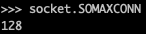
\includegraphics[width=\linewidth]{maxcon.png}
  \caption{Valor de SOMAXCONN.}
\end{figure}

\href{http://veithen.io/2014/01/01/how-tcp-backlog-works-in-linux.html}{Referência}

\section{Realize experimentos a fim de verificar quantos clientes conseguem de imediato
conectar-se ao servidor no passo anterior, comece com backlog em 0. Indique e
comprove a partir de qual valor de backlog as conexões não ocorrem imediatamente.
Elabore um esquema para tentar conectar 10 clientes de forma simultânea (Veja as
dicas logo abaixo).}

Foi criado um script \emph{run-multiple.sh} que realiza a compilação dos serviços e inicializa o servidor e 10 clientes conectados.

O servidor foi modificado para realizar um accept à cada 5 segundos com o uso de um \emph{sleep}, como forma de podermos observar quantos clientes conseguem se conectar instantaneamente para um dado \emph{backlog}.

Foi usado o comando \emph{sudo netstat -taulpn | grep PORT} para monitorar os estados da conexão TCP, onde conexões com o estado \emph{SYN\_SENT} não foram ainda movidas para a fila de accept, devido ela estar cheia.

Foi verificado que para à partir de \textbf{9} como valor no \emph{backlog}, todas as conexões iam para o estado \emph{ESTABLISHED} imediatamente, ou seja, todas as conexões couberam na fila de \emph{accept}.

\begin{figure}[H]
  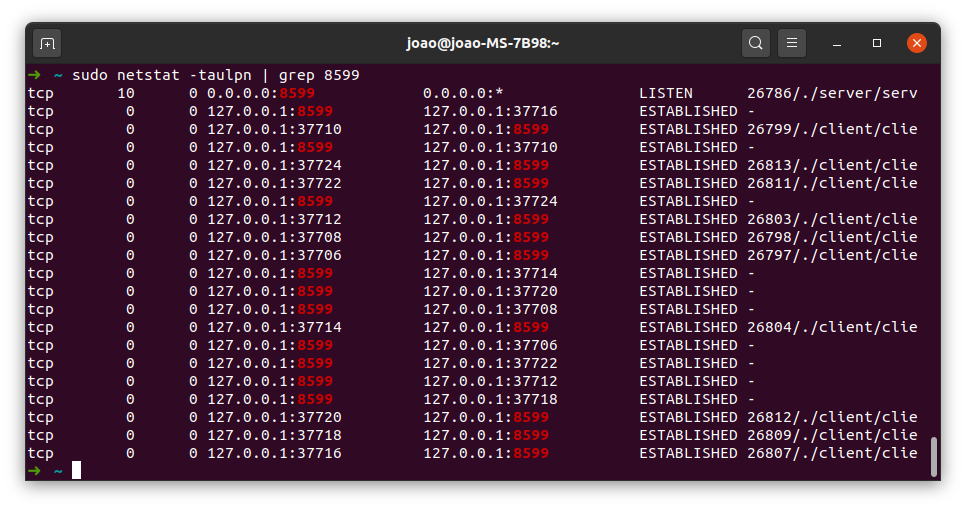
\includegraphics[width=\linewidth]{9-back.png}
  \caption{Resultado das conexões com 9 de backlog.}
\end{figure}

Para valores inferiores, conexões ficaram no estado \emph{SYN\_SENT} até mais conexões serem consumidas da fila de \emph{accept}

\begin{figure}[H]
  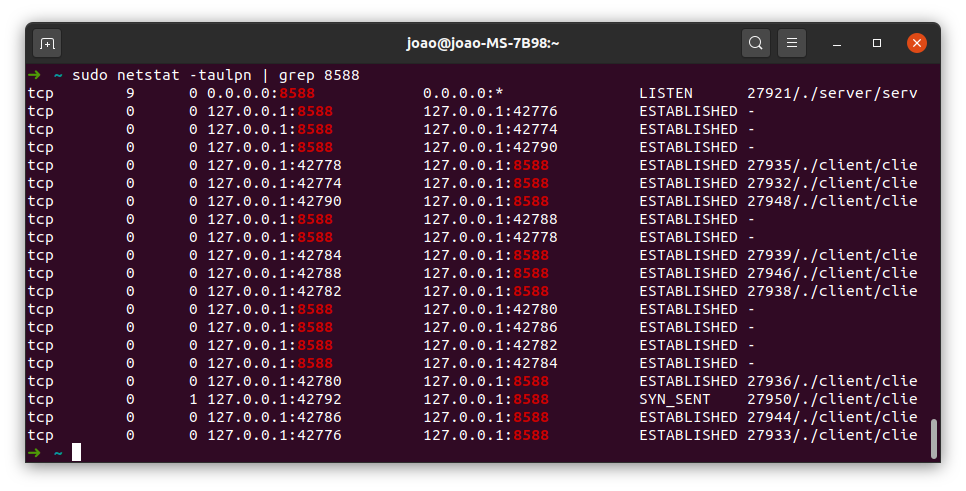
\includegraphics[width=\linewidth]{8back.png}
  \caption{Resultado das conexões com 8 de backlog.}
\end{figure}

Quanto menor o tamanho da fila definida pelo backlog, mais conexões ficam em estado incompleto inicialmente.

\begin{figure}[H]
  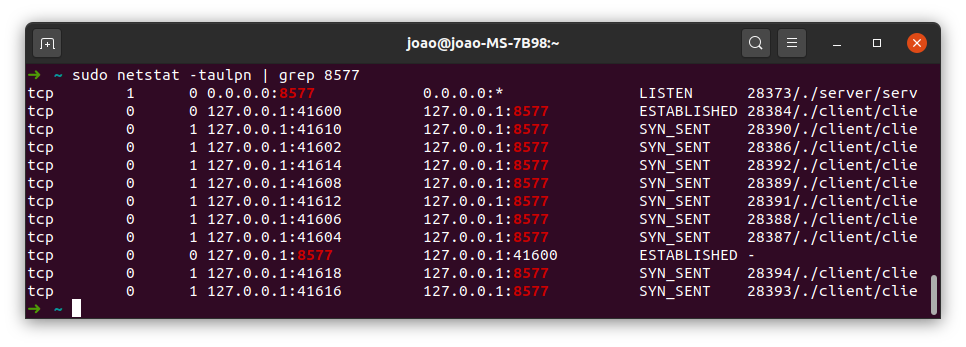
\includegraphics[width=\linewidth]{0back.png}
  \caption{Resultado das conexões com 0 de backlog.}
\end{figure}

\section{É correto afirmar que o código na versão atual gera processo zumbi? Explique. Se a
sua resposta foi sim, então altere o código da questão 3 de modo que os processos
criados pelo fork sejam corretamente finalizados ao invés de permanecerem no estado
zumbi quando um cliente encerra sua conexão.}

Na finalização de um processo filho, onde o sinal SIGCHILD é enviado, esse sinal não está sendo tratado no processo pai, então ficam processos zumbis para trás.

\bigskip

Então o servidor foi modificado para tratar o sinal \emph{SIGCHLD} no processo pai:


Então seja o processo do servidor pai com \emph{PID} \textbf{22873}, esses são os processos criados para os filhos:
\begin{figure}[H]
  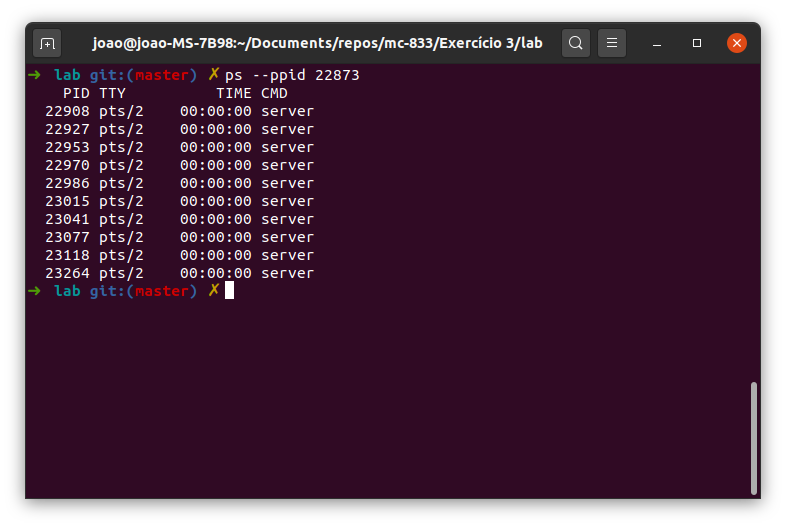
\includegraphics[width=\linewidth]{before.png}
  \caption{Processos filhos criados.}
\end{figure}

Então foi finalizado o cliente responsável pelo processo filho de PID \emph{23015}.

\begin{figure}[H]
  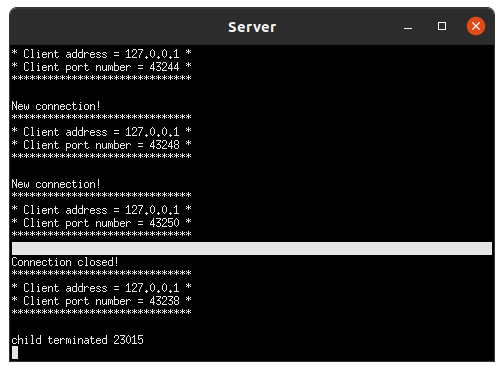
\includegraphics[width=\linewidth]{pa.png}
  \caption{Processo filho finalizado no servidor.}
\end{figure}


Então checando novamente os processos filhos, podemos notar que o processo foi removido, sem geração de processo zumbi.
\begin{figure}[H]
  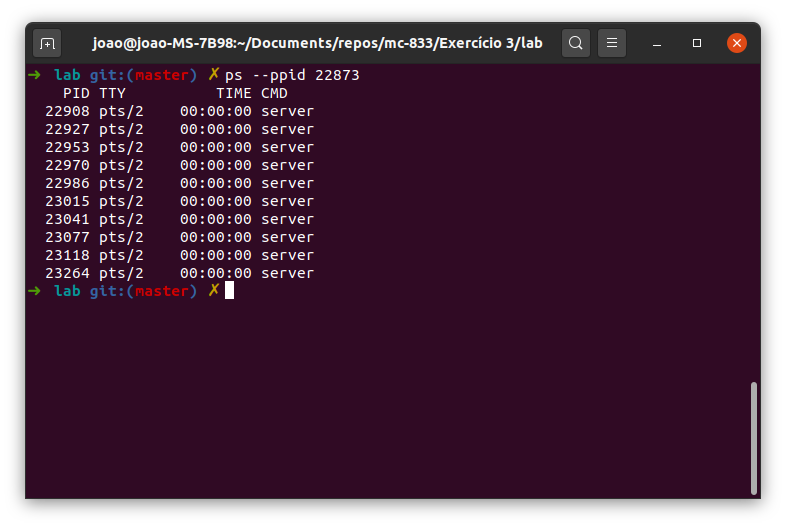
\includegraphics[width=\linewidth]{before.png}
  \caption{Processos filhos após finalização.}
\end{figure}

\section{Executando o trabalho}

Dentro da pasta \emph{lab}, basta executar o script \emph{run-multiple.sh}, que irá realizar a compilação do projeto (por meio do cmake), e irá executar em terminais separados (usando o xterm) o servidor e 10 outros clientes.

\bigskip

Para trocar a porta que será utilizada pela aplicação, basta alterar a linha do script contendo \emph{PORT=8577} por algum outro valor desejado.



% \subsubsection{Pseudocódigo}
% \begin{algorithm}
% \caption{InsertionSort(A)}
% \begin{algorithmic}[1]
%     \STATE $A[0] \longleftarrow -\alpha$
%   \STATE $i \longleftarrow 2 $
%     \FOR {$i$ to $N $} 
%             \STATE $j \longleftarrow i$

%             \WHILE{$A[j] > A[j-1]$} 
%                 \STATE $T \longleftarrow A[j-1]$ 
%                 \STATE $A[j-1] \longleftarrow A[j]$ 
%                 \STATE $A[j] \longleftarrow T$ 
%                 \STATE $j = j -1$
%             \ENDWHILE
%     \ENDFOR
%     \RETURN $A$
%     \end{algorithmic}
% \end{algorithm}




\end{document}